\section{Problem 2: Fine-Tuning ViT-B/32 on the PV Image Dataset}
\label{sec:p2}

%-------------------------------------------------------------------------
\subsection{Dataset, balancing and augmentation}
\label{sec:p2-data}

\paragraph{Dataset.}
The PV Image Dataset (InfraredSolarModules~\cite{millendorf2020pv}) contains 20{,}000 infrared images of single solar modules.
Each is a $40\times24$-pixel single-channel image labeled with one of 12 classes: 11 anomaly types and \emph{No-Anomaly}.
The classes are very imbalanced (\cref{tab:p2-balance}).
No-Anomaly has 10{,}000 images (50\%), while Diode-Multi has only 175 (0.9\%), a ratio of 57:1.

\paragraph{Pre-processing.}
We applied unsharp masking to every image, $\tilde x = x + a\,(x - G_r * x)$, where $G_r$ is a Gaussian blur and $a$ the sharpening amount.
This boosts local contrast and highlights the small hot spots and cell borders that separate the fault classes (\cref{fig:p2-samples}).
\TODO{state the radius $r$ and amount $a$ you used.}

\paragraph{Balancing.}
Every class was brought to exactly 2{,}500 images (\cref{tab:p2-balance}).
No-Anomaly, the only class above the target, was down-sampled at random: 7{,}500 images removed.
The 11 minority classes were up-sampled with 17{,}500 augmented images in total.
Each augmented image is a randomly chosen unsharpened original of that class, transformed by a random horizontal flip, a random vertical flip and a color jitter, which on a single-channel image changes brightness and contrast.
\TODO{state the jitter strengths.}
The balanced dataset has 30{,}000 images: 12{,}500 originals and 17{,}500 augmented copies.

\paragraph{Splits.}
We split each class 70/15/15 into train, validation and test \emph{by source image}: an original and all augmented copies made from it always fall into the same split.
A random split over all 30{,}000 images would put flipped copies of the same module into both the training and the test set and inflate the test accuracy.
Because the test set still contains augmented copies, we also report the test accuracy on its original images only.

\paragraph{Model input.}
Each $40\times24$ image is resized to $224\times224$ (bilinear), replicated to three channels and normalized with the ImageNet statistics.
With $32\times32$ patches, ViT-B/32 sees $7\times7=49$ tokens, each covering about $6\times3$ pixels of the original image.

\begin{table}[t]
  \centering
  \small
  \setlength{\tabcolsep}{4pt}
  \begin{tabular}{@{}lrrrr@{}}
    \toprule
    Class & Before & Removed & Augmented & After \\
    \midrule
    No-Anomaly     & 10{,}000 & 7{,}500 & 0       & 2{,}500 \\
    Cell           & 1{,}877  & 0       & 623     & 2{,}500 \\
    Vegetation     & 1{,}639  & 0       & 861     & 2{,}500 \\
    Diode          & 1{,}499  & 0       & 1{,}001 & 2{,}500 \\
    Cell-Multi     & 1{,}288  & 0       & 1{,}212 & 2{,}500 \\
    Shadowing      & 1{,}056  & 0       & 1{,}444 & 2{,}500 \\
    Cracking       & 940      & 0       & 1{,}560 & 2{,}500 \\
    Offline-Module & 827      & 0       & 1{,}673 & 2{,}500 \\
    Hot-Spot       & 249      & 0       & 2{,}251 & 2{,}500 \\
    Hot-Spot-Multi & 246      & 0       & 2{,}254 & 2{,}500 \\
    Soiling        & 204      & 0       & 2{,}296 & 2{,}500 \\
    Diode-Multi    & 175      & 0       & 2{,}325 & 2{,}500 \\
    \midrule
    Total          & 20{,}000 & 7{,}500 & 17{,}500 & 30{,}000 \\
    \bottomrule
  \end{tabular}
  \caption{Images per class before and after balancing. ``Removed'': random down-sampling of the majority class. ``Augmented'': flipped and color-jittered copies of unsharpened originals.}
  \label{tab:p2-balance}
\end{table}

\begin{figure}[t]
  \centering
  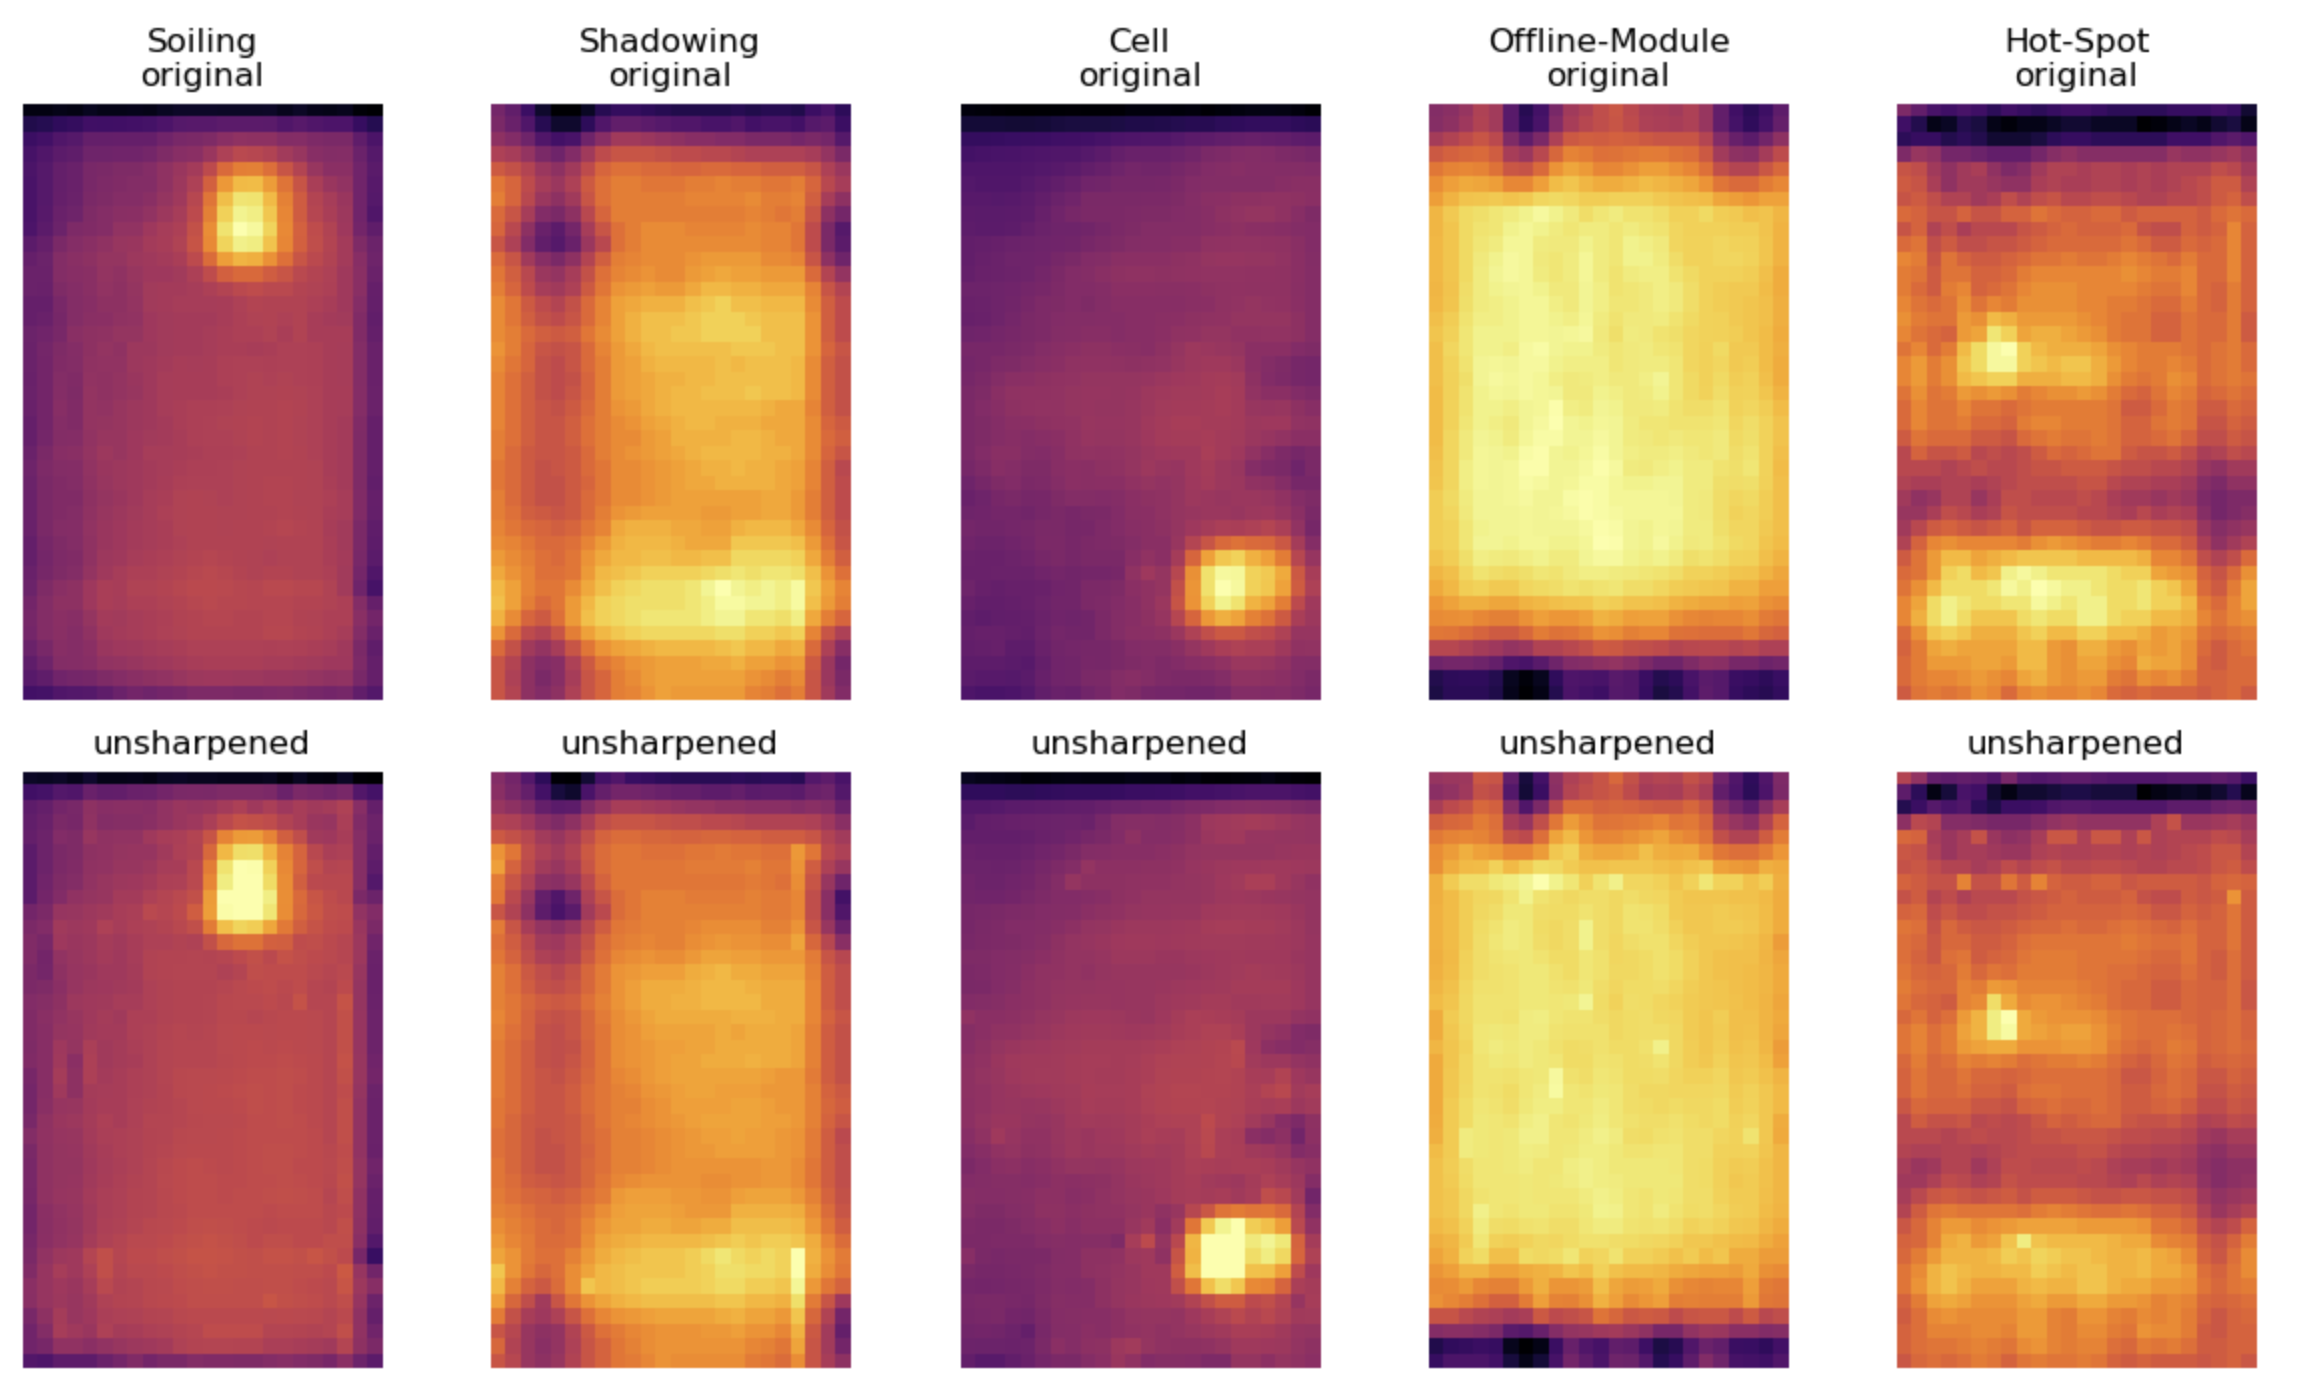
\includegraphics[width=\linewidth]{figs/p2_samples.png}
  \caption{Five sample images with their labels, before (top) and after (bottom) unsharp masking (false color, $40\times24$ pixels). Sharpening makes hot spots, cell borders and the shadow edge more distinct.}
  \label{fig:p2-samples}
\end{figure}

%-------------------------------------------------------------------------
\subsection{Fine-tuning strategies}
\label{sec:p2-train}

We fine-tuned the ImageNet-1k pre-trained ViT-B/32~\cite{dosovitskiy2021vit} from torchvision, with its classifier replaced by a new 12-way linear layer.
Three strategies differ only in which parameters are trained (\cref{lst:p2-freeze}):
(1) the classifier head only,
(2) the entire model, and
(3) the last four transformer blocks, the final layer norm and the head.
All runs use AdamW~\cite{loshchilov2019adamw} with weight decay 0.01 and a one-cycle learning-rate schedule with a 10\% warm-up, for 10 epochs with batch size 128 and bfloat16 mixed precision on one Sol GPU.
The peak learning rate is larger when fewer parameters are trained: $10^{-3}$ for the head, $10^{-4}$ for the last blocks and $5\cdot10^{-5}$ for the entire model, so the pre-trained weights are not destroyed.
We keep the epoch with the best validation accuracy and evaluate it on the test set.
Training time counts only the training passes, not the evaluation.

\begin{lstlisting}[caption={The three fine-tuning strategies (from \texttt{vit\_finetune.py}, lightly reformatted).},label={lst:p2-freeze},float=t]
m = vit_b_32(weights=ViT_B_32_Weights.IMAGENET1K_V1)
m.heads.head = nn.Linear(
    m.heads.head.in_features, 12)   # 12 PV classes
for p in m.parameters():
    p.requires_grad = False           # freeze all
last4 = list(m.encoder.layers)[-4:]
parts = {"head": [m.heads],
         "full": [m],
         "last": [m.heads, m.encoder.ln, *last4]}
for part in parts[strategy]:          # unfreeze
    for p in part.parameters():
        p.requires_grad = True
\end{lstlisting}

\begin{table*}[t]
  \centering
  \small
  \begin{tabular}{@{}lrrcccccc@{}}
    \toprule
    Strategy & \makecell[r]{Trainable\\parameters} & \makecell[r]{Trainable\\(\%)} & \makecell{Peak\\LR} & \makecell{Train\\acc.} & \makecell{Val.\\acc.} & \makecell{Test\\acc.} & \makecell{Test acc.\\(originals only)} & \makecell{Training\\time (min)} \\
    \midrule
    1) Classifier head only & 9{,}228 & 0.01 & $1\cdot10^{-3}$ & 60.76\% & 54.97\% & 56.31\% & 55.15\% & \textbf{1.3} \\
    2) Entire model & 87{,}464{,}460 & 100.00 & $5\cdot10^{-5}$ & 99.94\% & \textbf{71.83\%} & \textbf{73.25\%} & \textbf{76.37\%} & 4.2 \\
    3) Last 4 blocks + head & 28{,}362{,}252 & 32.43 & $1\cdot10^{-4}$ & 99.98\% & 67.34\% & 68.70\% & 72.48\% & 2.3 \\
    \bottomrule
  \end{tabular}
  \caption{ViT-B/32 on the balanced PV dataset: accuracy and training time of the three fine-tuning strategies (10 epochs; best-validation epoch).}
  \label{tab:p2-results}
\end{table*}

\begin{figure*}[t]
  \centering
  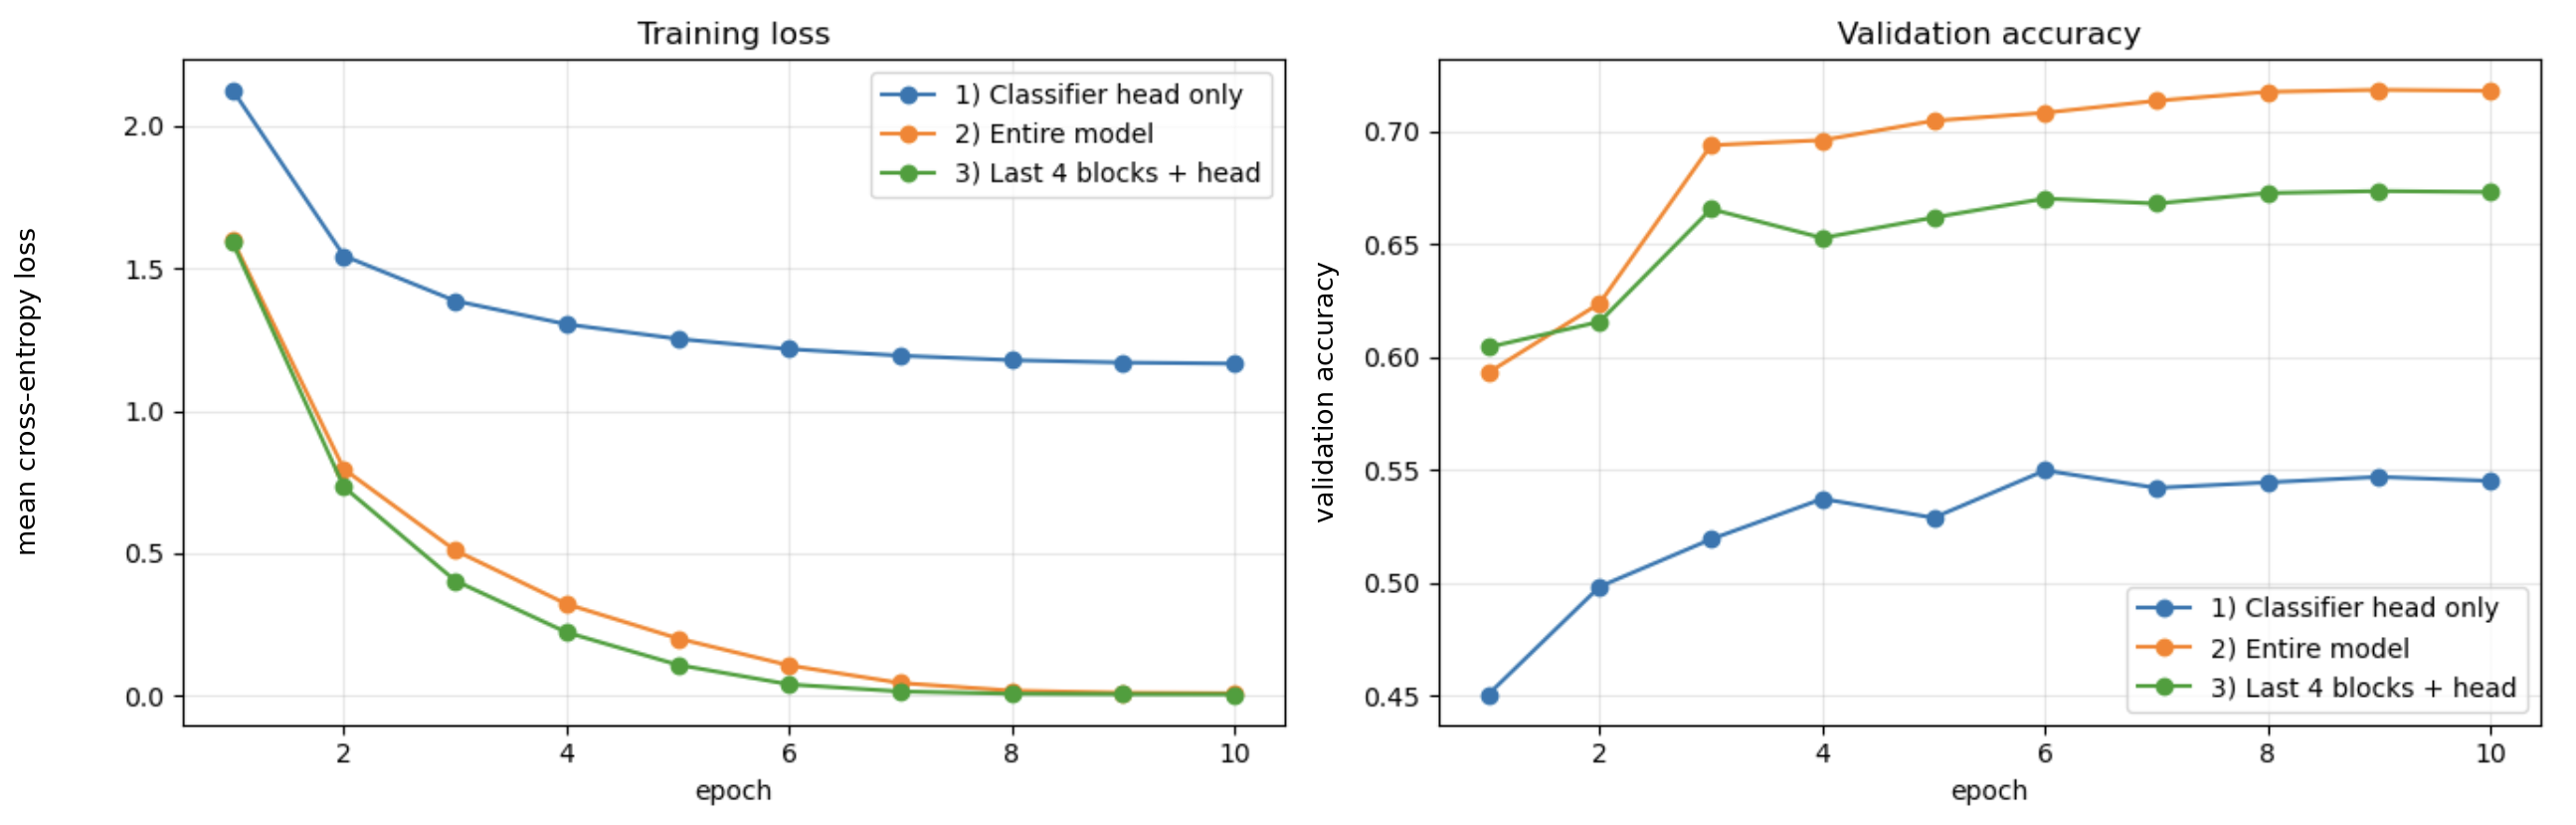
\includegraphics[width=0.9\textwidth]{figs/p2_curves.png}
  \caption{Training loss (left) and validation accuracy (right) per epoch for the three fine-tuning strategies.}
  \label{fig:p2-curves}
\end{figure*}

\paragraph{Results.}
\Cref{tab:p2-results} and \cref{fig:p2-curves} show the outcome.
Fine-tuning the entire model gives the best accuracy on every split: 73.25\% test, and 76.37\% on the original test images.
Fine-tuning the last four blocks reaches 68.70\%.
Training only the head reaches just 56.31\%, but takes only 1.3 minutes.

\paragraph{CNN reference.}
As an additional reference, we trained a ResNet-50~\cite{he2016resnet} on the same balanced dataset (\cref{tab:p2-resnet}).
\TODO{one sentence on what the improved version (\texttt{resnet2}) changes, and which transforms the test-time augmentation (TTA) averages over.}
The improved ResNet-50 with TTA reaches 72.6\% test accuracy (75.7\% on originals only), close to the fully fine-tuned ViT-B/32 (73.25\% and 76.37\%).
Without TTA, it is 2.5 points behind the ViT (70.8\%).

\begin{table}[t]
  \centering
  \small
  \begin{tabular}{@{}lcc@{}}
    \toprule
    Model & Test acc. & \makecell{Test acc.\\(originals)} \\
    \midrule
    ResNet-50 baseline & 67.2\% & 69.8\% \\
    ResNet-50 improved & 70.8\% & 73.6\% \\
    ResNet-50 improved + TTA & 72.6\% & 75.7\% \\
    \midrule
    ViT-B/32, entire model & \textbf{73.25\%} & \textbf{76.37\%} \\
    \bottomrule
  \end{tabular}
  \caption{ResNet-50 reference results on the same dataset (baseline: \texttt{resnet}; improved: \texttt{resnet2}; TTA: test-time augmentation), compared with the best ViT-B/32 strategy of \cref{tab:p2-results}.}
  \label{tab:p2-resnet}
\end{table}

%-------------------------------------------------------------------------
\subsection{Analysis}
\label{sec:p2-analysis}

\paragraph{Effect on performance.}
\begin{itemize}[nosep,leftmargin=*]
  \item \emph{Head only underfits.} Its training accuracy is only 60.8\%, and its training loss levels off at about 1.2 (\cref{fig:p2-curves}). The frozen ImageNet features are not linearly separable for these fault types. The domain gap is large: the inputs are single-channel thermal images upsampled 5.6--9.3 times, so they are very smooth and have none of the color and texture statistics of ImageNet photos, and the classes differ by small hot-spot patterns.
  \item \emph{Unfreezing blocks lets the model build infrared-specific features.} Training the last four blocks adds 12.4 points of test accuracy. Training the entire model adds another 4.6 points, because the early blocks and the patch embedding also adapt to the low-level statistics of the thermal images.
  \item \emph{Both deeper strategies overfit.} They reach $\approx$100\% training accuracy, but validation accuracy stays at 67--72\%, a gap of about 30 points, and after epoch 3 it improves by only 2--3 more points while the training loss keeps falling to zero. The likely reason is the up-sampling: a minority class such as Diode-Multi has only $\approx$120 training originals, each repeated about 14 times as flipped or jittered copies, so the model can memorize them. Stronger regularization (mixup, RandAugment, stochastic depth), a class-balanced loss instead of heavy oversampling, or ViT-B/16, which gives tiny images four times more tokens, are natural next steps.
  \item \emph{Originals-only accuracy is higher} for both deeper strategies (76.4\% vs.\ 73.3\% for the entire model). Augmented images exist only for the 11 minority classes, which are the hardest, so the full test set weights these classes more heavily than the originals do.
\end{itemize}

\paragraph{Effect on training efficiency.}
Training time grows with the number of parameters that receive gradients: 1.3, 2.3 and 4.2 minutes.
The head-only run trains almost 10{,}000 times fewer parameters but is only 3.2 times faster, because every epoch still runs the full forward pass through the frozen network.
Caching the frozen features once would make it almost free.
Training the last four blocks skips the backward pass through the first eight blocks and keeps optimizer states for only 32\% of the parameters.

\paragraph{Best trade-off.}
Fine-tuning the last four blocks gives the best accuracy per unit of training time.
It obtains 73\% of the accuracy gain of full fine-tuning over head-only training (12.4 of 16.9 points) for 34\% of the extra training time (1.0 of 2.9 minutes) and with a third of the trainable parameters.
For this small dataset, however, full fine-tuning costs only 4.2 minutes and is clearly the most accurate, so it is the strategy we would choose.
The partial strategy becomes the better choice for larger models or datasets, where full fine-tuning is expensive in time and memory.
